\section{A WSN with Waspmotes: Theoretical aspects}
\label{Chapter3}
\subsection{Introduction}
Waspmote is more than just another piece of hardware. In fact it is an open source platform for wireless sensors, specially focusing on low consumption and autonomy. Waspmotes promise to offer a variable lifetime between 1 and 5 years, depending on the duty cycle and the used radio.\\ 
But it didn't just start with Waspmote and it will definitely not end with it. In 2007 developers from Libelium collaborated with the Arduino Team creating the first open hardware shield for Arduino, the "Arduino XBee Shield" \defcitealias{SHIELD}{Arduino Team, 2012}\citepalias{SHIELD}. The shield allowed an Arduino board to communicate wirelessly via ZigBee. Libelium used the shield to develop their first sensor device, the SquidBee, intended for creating sensor networks. Although the SquidBee is self-powered and implements wireless communications, it is more sensor device than wireless sensor device. The 3.3V - 5V regulator could not be turned off, as a result there is a constant consumption of 50mA discharging the battery within hours. The SquidBee was created for teaching and educational purposes only \defcitealias{SQUID}{Libelium, 2009}\citepalias{SQUID}. Since the platform was not radio certified the motes could not be deployed in real scenarios like cities, factories or even houses, so it did not fit Libelium's corporate customer requirements at all. However, the tone of an open hardware and source wireless sensor device was definitely set.
\begin{figure*}[ht]
\centering
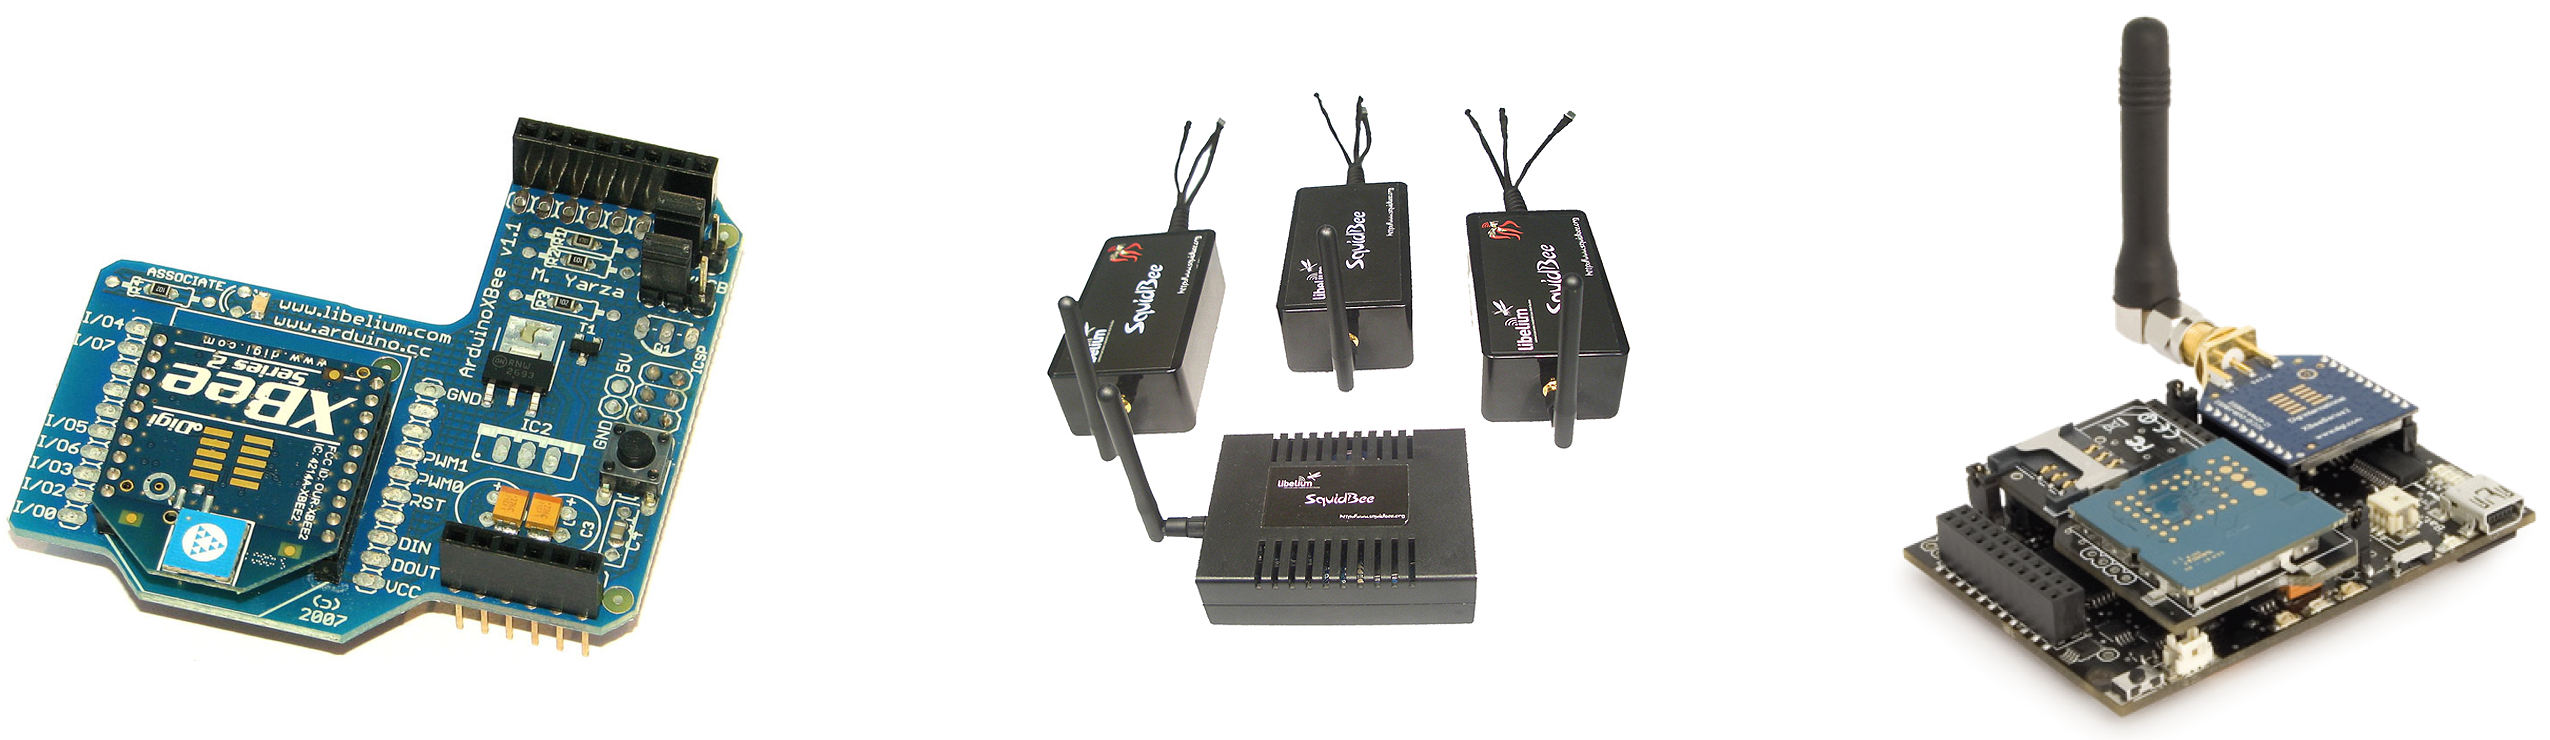
\includegraphics[width=0.98\textwidth]{chap3}
%\rule{30em}{0.5pt}
\caption{Waspmote going from ON to Deep Sleep}
\label{fig:chap3}
\end{figure*}\\
In 2009 the Waspmote was born, meeting all the above requirements: low consumption and meeting three radio certification requirements (CE for Europe, FCC for the US and IC for Canada). In addition the Waspmote was built with a complete modular philosophy. The idea behind this design is to integrate only the needed modules in each device, optimizing costs. This is why all modules are connected to the Waspmote via sockets\defcitealias{CH}{Cooking Hacks, 2013}\citepalias{CH}.\\Since its introduction, more than 2000 developers have been using Waspmote (v1.1) and the platform has received many suggestions and possible improvements. Libelium carefully listened to all these proposals and decided to bring out a new version with the name of Waspmote PRO (v1.2) in February 2013 \defcitealias{NEW}{WSN Research Group, 2013}\citepalias{NEW}. This new version comes with upgraded hardware and improved API, which is unfortunately not compatible with the older API. The most important improvements of the hardware is that the code can be uploaded much quicker and the XBee radio must no longer be removed to do so. A new interrupt enables the XBee to wake the Waspmote PRO whun XBee cyclic sleep modes are used \defcitealias{PRO}{Waspmote (v1.1) vs Waspmote PRO (v1.2), 2013}\citepalias{PRO}. To do this on the old version one must solder pin 13 of the XBee to the MUX\_RX pin of the Waspmote. This way interruptions caused by the XBee module can be captured, but all other interruption options (RTC, ACC, etc.) will be masked by the XBee 13 pin output and thus will be lost.  The new version also no longer has jumpers and there is no need of a coin battery. Regarding the API, Libelium claims it is much more robust and easier to use than the previous one and they also improved their programming guides. One big feature of the new API is the support to send AT commands to the XBee.
%----------------------------------------------------------------------------------------
\subsection{Hardware}
\subsubsection{Modular Architecture}
As mentioned in this chapter's introduction, Waspmote is based on a modular architecture, doing so optimizing costs and able to change according to the specific user's requirements. The available modules are split up into five categories:
\begin{itemize}
\item ZigBee
\item GSM - 3G/GPRS
\item GPS
\item Sensor Boards
\item Storage
\end{itemize}  
Figure \ref{fig:waspMote1} indicates the Waspmote main components.
\begin{figure}[ht]
\centering
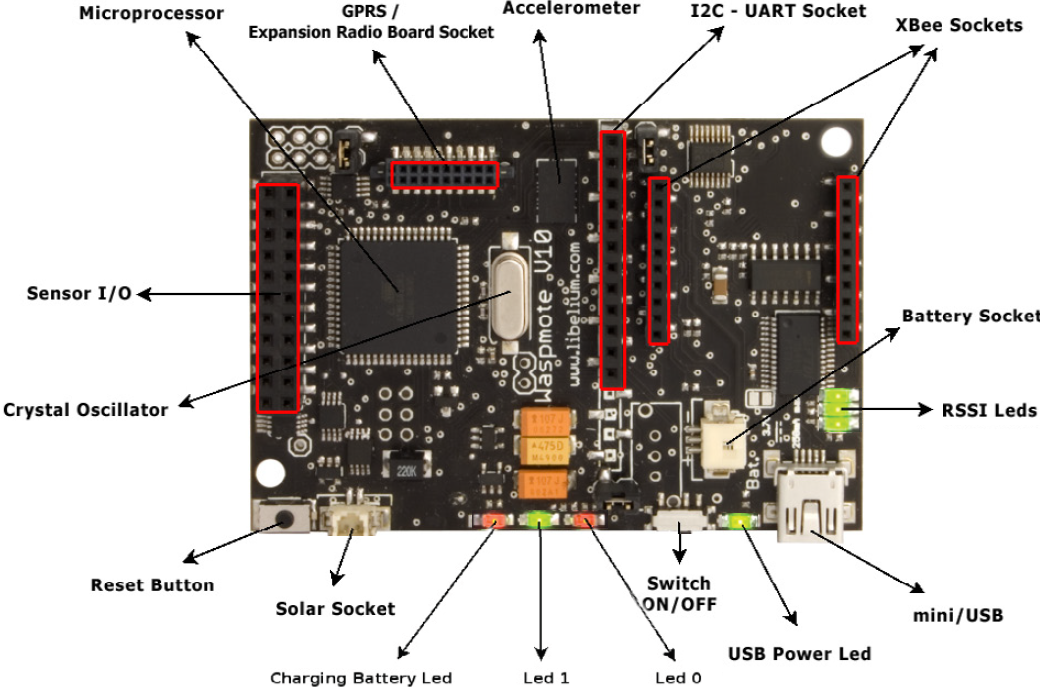
\includegraphics[width=0.48\textwidth]{waspmote2}
%\rule{30em}{0.5pt}
\caption{Main Waspmote components}
\label{fig:waspMote1}
\end{figure}
%-------------------------------------------
\subsubsection{Microcontroller and memory}
\label{memory}
Because of the modular design of the Waspmote the block diagram (see figure \ref{fig:block} \label{fig13}) is very simple. Just like on any other PCB, the CPU is the heart of the module. Waspmote integrates an 8-bit ATmega 1281 microcontroller with 128KB programmable flash, 8KB SRAM runtime memory and 4KB EEPROM memory. Since SRAM is is built with cleverly combined MOSFETs it must not be periodically refreshed, but it is still volatile memory. The main advantage compared to DRAM is that, when moderately clocked like in the Waspmote, it consumes very little power.\\
The AVR was developed in 1996 by Atmel. It is a modified Harvard architecture 8-bit RISC microcontroller and was one of the first microcontroller families to implement flash memory for program storage (opposed to other microcontrollers at the time that were using 1-time programmable ROM, EPROM or EEPROM).\\
A Harvard computer architecture has separate storage and signal pathways for instructions and date. It can fetch instructions and data at the same time and can thus be faster than pure von Neuman architecture. Systems can have much more instruction memory than data memory, so instruction address zero might indicate a 24-bit value for a 16-bit instruction, while data address zero might identify an 8-bit value for 8-bit wide data. Since most AVR instructions are 16 bit wide, the flash memory of the ATmega1281 with 128KB is organized as 64K x 16, so the Program Counter is 16 bits wide \defcitealias{ATMEGA}{Atmel ATmega 1281 Datasheet, 2012}\citepalias{ATMEGA}.\\
The architecture of the ATmega microcontroller is modified Harvard but the separate address space nature of a Harvard machine is preserved. In contrast to systems that add CPU cache, in which data and instructions are unified, providing the von Neumann model. The adaptation is much more subtle. The ATmega has an Extended Load Program Instruction which can allocate constant tables within the program memory address space (see figure \ref{fig:architecture} \label{fig14}). So the contents of the instruction memory can be accessed as data, saving scarce runtime memory. This creates however certain difficulties in programming, since the C Language was not designed for Harvard architectures (see section \ref{memory}). 
%-------------------------------------------
\subsubsection{Timers}
The Waspmote's system clock is an 8MHz quartz oscillator. This means that every 125ns a machine language instruction is executed by the microcontroller. Keep in mind that one C++ instruction consists of several instructions in machine language. To generate interrupts the Waspmote has an internal watchdog and a Real Time Clock (RTC).
\paragraph{Watchdog}
The Watchdog is integrated on the Atmega 1281 and counts the clock cycles generated by a 128KHz oscillator. When the WDT counter reaches a set value it generates an interruption signal. The WDT is used to awake the microcontroller from \textit{Sleep} mode, because of its high precision. Thus, \textit{Sleep} mode allows small intervals, going from 16 milliseconds to a maximum of 8 seconds.
\paragraph{Real Time Clock}
To store an absolute time base the RTC can be used. Alarms programmed in the RTC specify days, hours, minutes and seconds. For the RTC the waspmote uses a Maxim DS3231SN 32.768Hz oscillator. Because this clock has an internal compensation mechanism for variations caused by temperature changes this is one of the most accurate clocks on the market. This clock is used to wake the Waspmote from the higher energy saving modes \textit{Deep Sleep} and \textit{Hibernate}, with intervals from 8 seconds to even days. It is important to notice that in \textit{Hibernate}, the RTC is no longer powerd through the main battery but through the auxiliary (button) battery. So when problems occur when using hibernate probably it is recommended to measure the button battery's voltage and possibly must be replaced.
%----------------------------------------------------------------------------------------
\subsection{Programming}
To develop on the Waspmote, Libelium offers an API and IDE. For more information on the API, please see section \ref{LibAPI}. Waspmote uses the same IDE (compiler and core libraries) as Arduino, so as long as things like pin layout and I/O schemes are adjusted, code should be compatible in both platforms. So Waspmote and Arduino are pretty much the same, however don't forget that Waspmote has Radio Certifications and Arduino doesn't.\\  
When the Waspmote is started, the microcontroller will execute the bootloader and start loading the compiled program from FLASH into the SRAM working memory.\\
The code is divided into two basic parts: \textbf{setup} and \textbf{loop}, each with sequential behaviour. When the Waspmote is switched on or reset, the code starts at the setup function and then enters the loop function. Because the second part forms an infinite loop a common technique to save energy is to block the program until some interruption is detected.\\
Since in \textit{Hibernate} mode the Waspmote is completely disconnected from the main battery also the program is interrupted. This means the SRAM has lost all variable values and at wake up the code restarts at the \textbf{setup} function. To store values during hibernate cycles it is necessary to write them to EEPROM or to the SD card.
%----------------------------------------------------------------------------------------
\subsection{Power considerations}
\label{pow}
\subsubsection{Waspmote power modes}
\label{dynPow}

from intro:

Waspmotes have a very low power consumption in \textit{Hibernate} mode but for shorter sleep times and the conservation of program variables \textit{Deep Sleep} mode is more advisable. Unfortunately it is not easy to combine and switch between the modes depending on the next time to sleep.\\
Although OTA programming is supported on Waspmotes, it should be limited to a minimum in order to obtain reasonable battery durations. Writing to FLASH takes about 83nAH per byte, whilst reading only takes 1.1nAH per byte \citep{KTH}. 


\paragraph{PHY Layer Responsibilities}
\begin{itemize}
\item Enabling and disabling the radio transceiver ... ...
\item Transmit and receive data ... ...
\item Select CH ... ...
\item Estimating signal energy ... ...
\item Providing RSSI, LQI ... ...
\end{itemize}
\paragraph{MAC Layer Responsibilities}
\begin{itemize}
\item Generating beacons ... ...
\item CSMA-CA, BPSK vs. O-QPSK, vs. ASK ... ...
\item Providing a reliable link ... ...
\item PAN association and disassociation services
\end{itemize}
\paragraph{Network Layer Responsibilities}
\begin{itemize}
\item Setting up a network ... ...
\item Allow joining and leaving a network ... ...
\item Configuring new devices ... ...
\item Discover and maintain routes ... ...
\end{itemize}
\paragraph{Application Layer Responsibilities}
\begin{itemize}
\item Application support ... ...
\item Address management and mapping ... ...
\item Define the role of the device ... ...
\item Security related tasks ... ...
\end{itemize}
%-----------------------------------------
\subsection{Networking concepts}
\subsubsection{Device Types}
\subsubsection{Device Roles}
In table \ref{fig:roles} from \defcitealias{DYNAMIC}{Dynamic C: An Introduction to ZigBee User Manual, 2008}\citepalias{DYNAMIC} an overview of the device responsibilities on network layer is given. 
\paragraph{Coordinator Operation}
\paragraph{Router Operation}
\paragraph{End Device Operation}
sleep...
\subsection{Parent - Child relationship}


The libelium Waspmote has 4 operational modes: ON, Sleep, Deep Sleep and Hibernate. They differ from which type of interruptions they can be woken up and duration interval. For our application we want sleep intervals of 30 seconds and more, so only Deep Sleep and Hibernate mode are of interest. Table \ref{tab:cons1} summarizes the Waspmotes operational modes.
\begin{table*}[!ht]
\begin{center}
\begin{tabular}[!ht]{|c|c|c|c|c|}
\hline
\textbf{Mode} & \textbf{Consumption} & \textbf{CPU} & \textbf{Cycle} & \textbf{Accepted Interruptions}\\
\hline
ON & 9mA & ON & - & Synch and Asynch\\
\hline
Sleep & 62$\mu$A  & ON & 31ms - 8s & Synch (WDT) and Asynch\\
\hline
Deep Sleep & 62$\mu$A & ON & 8s - min/hours/days & Synch (RTC) and Asynch\\
\hline
Hibernate & 0.7$\mu$A & OFF & 8s - min/hours/days & Synch (RTC)\\
\hline
\end{tabular}
\caption{Operational modes of Libelium Waspmote V1.1}
\label{tab:cons1}
\end{center}
\end{table*}
\paragraph{Deep Sleep}
In deep sleep mode the main program is paused and the CPU passes to a latent state. Triggers are as well synchronous interruptions (RTC) as asynchronous interruptions. Examples of asynchronous interruptions are low battery level or a sensor that reaches a certain trigger value.\bigskip
%\begin{figure}[ht]
%\centering
%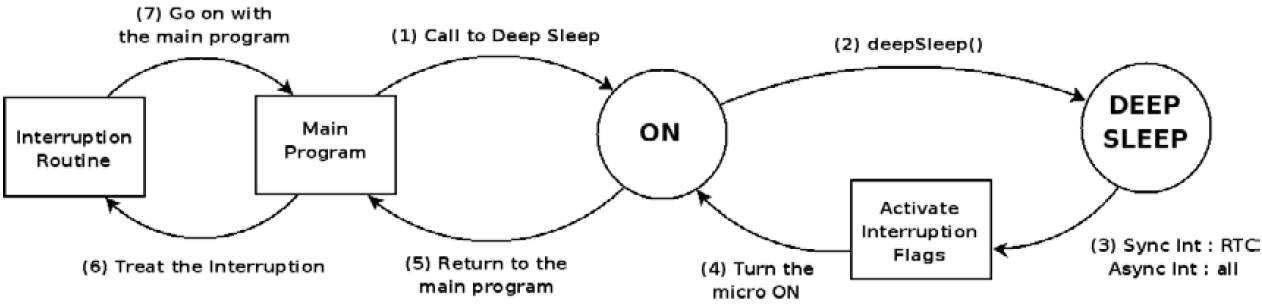
\includegraphics[height=3cm]{deepSleep}
%\rule{30em}{0.5pt}
%\caption{Waspmote going from ON to Deep Sleep}
%\label{fig:deepSleep}
%\end{figure}\bigskip
\\In figure \ref{fig:deepSleep} the process from going to operational mode ON to Deep Sleep is shown. The main advantage of this mode is that the program is only paused, so the program stack and thus all variable values keep their values. When the Waspmote is turned back on it simply executes the next instruction.
%-------------------------------------------
\paragraph{Hibernate}
Hibernate mode consumes roughly 100 times less energy than Deep Sleep. This is made possible by disconnecting all the Waspmote's modules, including the microcontroller. The RTC gets his power through the auxiliary battery. So if hibernate mode stops working it is probably necessary to replace the Waspmote's button battery. Figure \ref{fig:hibernate} demonstrates the process from ON to hibernate.\\
\begin{figure*}[ht]
\centering
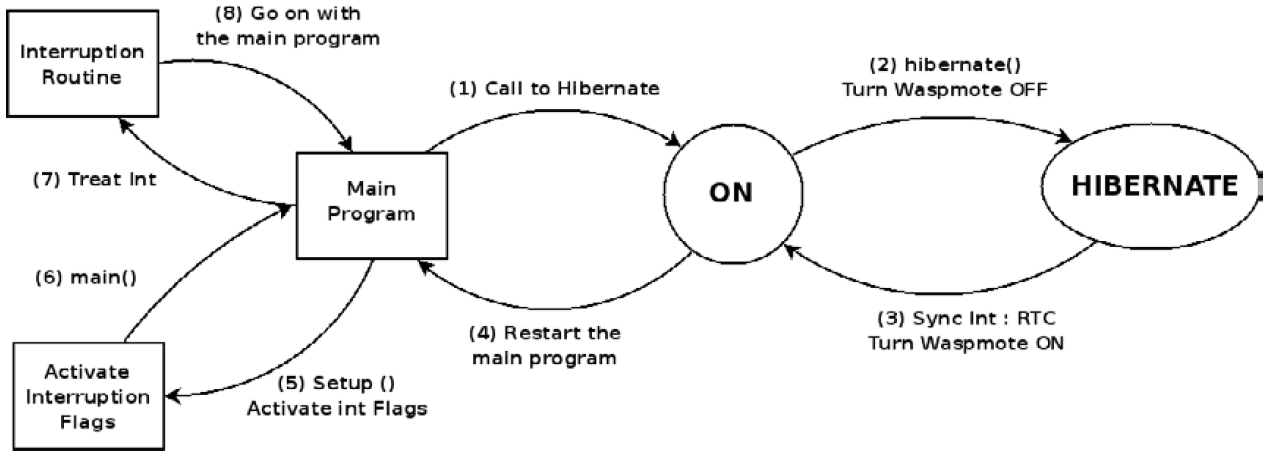
\includegraphics[width=0.74\textwidth]{hibernate}
\caption{Waspmote going from ON to Hibernate}
\label{fig:hibernate}
\end{figure*}
\begin{figure*}[!ht]
\centering
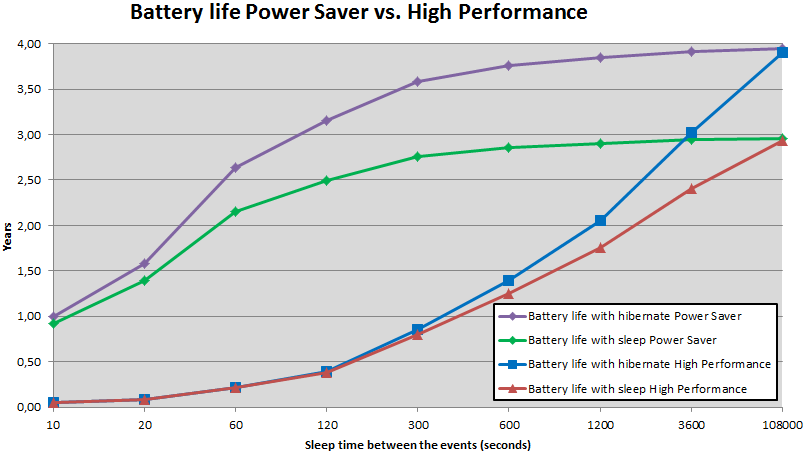
\includegraphics[width=0.86\textwidth]{battery2}
%\rule{30em}{0.5pt}
\caption{Battery life High Performance vs. Power Saver}
\label{fig:batCalcPS}
\end{figure*}
This means the CPU is also switched of and does not remember any values from variables. When waking up the Waspmote reinitializes, the microprocessor is reset and the program restarts from the beginning. Both \textbf{setup} and \textbf{loop} routines are executed as if the main switch would be activated. By placing the \verb+ifHibernate()+ function in setup the program can determine if it came from a hardware reset or from a hibernate reset. To be able to wake up from hibernate mode the hibernate jumper must be removed correctly. See section .... for remarks on this issue. \\Because not all Libelium's API functions regarding hibernate in combination with the different alarm modes work, it is advised to use the functions provided in \textbf{WaspXBeeZBNode.h}. 
%----------------------------------------------------------------------------------------
\subsubsection{Sampling sensors}
To measure the sensors, originally we took 10 samples with 100 milliseconds recommended delay between the measurements and calculated the average. Since we want to make the energy consumption as low as possible we now do the iterations without delay. Appendix \ref{sensMeasuring} contains 60 test samples per sensor and indicates that there is no significant difference on the average by removing this delay. Except for CO$_{2}$ measurements, removing the delay saves about 1000 milliseconds per measured sensor.\\ 
Because the first sample often shows a slight deviation, the program takes 11 samples but bases the average on the last 10 values.
%-------------------------------------------
\subsubsection{Battery life estimation}
In order to be able to give recommended sensor measuring intervals this section will analyse the estimated battery life of the Waspmotes. Table \ref{tab:cons2} enumerates the most common components typical consumption.
\begin{table}[!ht]
\begin{center}
\begin{tabular}[!ht]{|c|c|}
\hline
\textbf{Action} & \textbf{Average Current}\\
\hline
XBee, sending, & 105mA\\
\hline
CO$_{2}$ & 50mA\\
\hline
XBee, ON & 45mA\\
\hline
Waspmote, ON & 9mA\\
\hline
Pressure & 7mA\\
\hline
Humidity & 380$\mu$A\\
\hline
Waspmote, sleep & 62$\mu$A\\
\hline
Temperature & 6$\mu$A\\
\hline
Waspmote, hibernate & 0,007$\mu$A\\
\hline
\end{tabular}
\caption{Operational modes of Libelium Waspmote V1.1}
\label{tab:cons2}
\end{center}
\end{table}
The batteries included with our Waspmotes are rechargeable Lithium-ion batteries with a capacity of 6600mAH. The Waspmote that will be deployed on the roof of Group T, campus Vesalius will also have a 12V solar panel with a charging current up to 280 mA to extend its battery life. The other batteries can by charged manually or by USB (5V, 100mA). Lithium-ion have a self-discharge rate of typcially 1 to 2 percent per month \citep{LION} and since the used batteries are new we expect a high battery efficiency.\\
%-------------------------------------------
\paragraph{XBee and Waspmote start-up times}
\label{startup}
For the XBee node to join an existing network there are two power related possibilities. Either the Waspmote has been turned on already sufficiently long and the XBee had more than enough time to join the network, or either the XBee wasn't joined yet and the program needs to wait on this. From the experiments done at our apartment we came to following conclusions:
\begin{enumerate}
\item It takes about 2.5 seconds to join a network after powered on.
\item If the XBee is joined, the program still needs to confirm this. This takes 452 milliseconds.
\item The sending time is constant, about 158 ms, if the XBee had more than 2.5 seconds to join. However in case the XBee must send immediately after it is joined, the sending time is not constant and takes on average 611 milliseconds.
\item The sending time increases if there are more obstructions between the antennas. 
\end{enumerate}
With these characteristics we came to results discussed in the next sections. For the validation of these conclusions please see appendix \ref{AppendixA}. Table \ref{tab:sendTime} sums up the results of the distance-relation test.
\begin{table}[!ht]
\begin{center}
\begin{tabular}[!ht]{|c|c|}
\hline
\textbf{Distance} & \textbf{Average sending time (ms)}\\
\hline
Air & 158\\
\hline
1 Floor & 268\\
\hline
2 Floors & 357\\
\hline
3 Floors & 484\\
\hline
4 Floors & 558\\
\hline
5 Floors & unreachable\\
\hline
\end{tabular}
\caption{Distance consequence on send times}
\label{tab:sendTime}
\end{center}
\end{table}\\
To save power the Waspmote can store the values for a user determined time. Taking samples and save them to EEPROM in case of hibernate mode takes only 6 - 7\% of the time to measure and send. Table \ref{tab:sendTime3} confirms this.
%-------------------------------------------
\paragraph{Battery life with standard program optimizations}\label{batLife1}
The application scenario for this battery test is as follow: the Waspmote will be turned on as short as possible and 4 sensors, namely temperature, humidity, pressure and battery level will be sampled. The node will take 10 samples for each sensor and calculate the average. Those values are put into one ZigBee packet and sent to the gateway. By adapting the sleep time between the event we came to the rather disappointing results shown in figure \ref{fig:batCalcHP}.\\ The graph in figure \ref{fig:batCalcHP1} breaks down the total energy consumption to five categories. It shows the monthly energy consumption as a function of the time between the events. For small intervals the active energy usage is huge. Only starting at 20 minutes sleep time the self-discharge becomes dominant and from 3 hours on the sleep mode current also becomes dominant.\\
Since the Waspmotes use this much energy when applied this way we will call this the High Performance mode from now on. The next section calculates an alternative approach, referred to as Power Saver mode. This nomenclature is continued in the program:
\usestyle{vs} %other useful styles are, bw,  borland, vs
% Include the source code 
\includecode{pp.cpp}
%\begin{minted}{c++}
%typedef enum{HIGHPERFORMANCE, POWERSAVER} 
%PowerPlan; 
%\end{minted}
%-------------------------------------------
\paragraph{Battery life with extra optimizations}
\label{powerSaver}
As shown earlier in this section, sending values requires that the Waspmote is on for at least 3 seconds. In addition the XBee uses about five times the energy of the Waspmote. For end devices it is obviously recommended to turn on the XBee as little as possible, within a user defined limit.\\ Figure \ref{fig:batCalcPS} shows the same results as the application scenario discussed in section \ref{batLife1} and adds the results for a mode further referred to as Power Saver.\\
The implementation of this mode will depend on the nodes sleep settings. For \textit{Deep Sleep} the values can simply be stored on the heap, but for \textit{Hibernate} the values must be written to EEPROM.\\
Because of the size limit of a ZigBee packet we can store maximum 30 values and send them in one packet. However, if the sensor measuring interval is small the user can opt to store more values and send two or more packets after each other. The values for Power Saver in table \ref{tab:cons2} are of an example scenario that takes 60 measurements and then sends them in two packets to the gateway. It are also those results which are put in function of time in figure \ref{fig:batCalcPS}.\\
As visible on figure \ref{fig:batCalcPS} \textit{Hibernate} has more influence in Power Saver mode, already extending battery life significantly at a 20 seconds interval comparing to a 10 minutes interval in High Performance mode. Also the energy breakdown graph in figure \ref{fig:batCalcPS1} shows that the interval times must be increased much less before the dominant factor is self-discharge and sleep mode energy consumption, compared to figure \ref{fig:batCalcHP1}.\\By reducing the sensor measurement accuracy battery life can be extended with modest 3 - 4\%, best case scenario. Please see appendix \ref{appendixA} for details.\\
In case the measuring intervals are small it is recommended to use \textit{Deep Sleep} instead of \textit{Hibernate}, since in hibernate the values are written to EEPROM. Equation \ref{eq:1} shows this can be very destructive for the Waspmote. Depending on how much freedom the user is given, the program can make the decision to switch to \textit{Deep Sleep} on itself, or the installation's administrator can control this.
%-------------------------
\subsubsection{Sleeping Mesh}
What is \textit{really} low power about ZigBee? The answer is already deducible from the previous sectionsn, namely End Devices! A sleeping mesh tries to establish a multi-hop mesh network and low power routing functionality in one system, also using battery-powered routers. The system has two big requirements however:
\begin{itemize}
\item very low bandwidth, high latency
\item static network
\end{itemize}
For example, delivery of one data packet from every node every 12-24 hours, with a wake period of about 15 seconds. In a sleeping mesh all nodes wake up simultaneously and periodically to exchange and or route data. Afterwards, all nodes except the coordinator go back to sleep, a state which they are in 99\% of the time. In such a set-up battery lifes of 10 years and more are easy to reach.